\documentclass{article}
\usepackage{graphicx}
\usepackage[pdftex]{hyperref}
\usepackage{color}

\newcommand{\martin}[1]{\marginpar{\textcolor{magenta}{\textbf{Martin: }#1}}}
\newcommand{\imartin}[1]{\textcolor{blue}{\textbf{Martin: }#1}}


\begin{document}
\title{Using SLA's to guide database transition to NoSQL on the cloud: a systematic mapping study}
\author{Fabio Leal $\langle$\href{mailto:sousaleal.fabio@gmail.com}%
{sousaleal.fabio@gmail.com}$\rangle$
\\
Martin A. Musicante $\langle$\href{mailto:mam@dimap.ufrn.br}%
{mam@dimap.ufrn.br}$\rangle$}
\date{\today}
\maketitle  




\begin{abstract}
Cloud computing became a reality over the last years, and many companies are now moving their data-centers to the cloud. 
A concept that is often linked with cloud computing is Infrastructure as a Service (IaaS): the computational infrastructure of a company can now be seen as a monthly cost instead of a number of different factors. 
Recently, a large number of organizations started to replace their relational databases with hybrid solutions (NoSQL DBs, Search Engines, ORDBs). 
These changes are motivated by (\textit{i}) performance improvements on the overall performance of the applications and (\textit{ii}) inability to a RDBMS to provide the same performance of a hybrid solution given a fixed monthly infrastructure cost. 
However, not always the companies can exactly measure beforehand the future impact on the performance on their services by making this sort of technological changes (replace RDBMS by another solution). 
The goal of this systematic mapping study is to investigate the use of Service-Level-Agreements (SLA’s) on database-transitioning scenarios and to verify how SLA’s can be used in this processes.
\end{abstract}

\section{Introduction}

The adoption of cloud solutions is growing fast among organizations~\cite{6546068}.
Centralized (mostly mainframe) technology is being replaced by distributed and more flexible forms of data storage and processing.
This change of paradigm is motivated by the necessity to improve the use of resources, as well as by the increasing velocity in which data is produced.

In this scenario, transitions must take into account the quality of the service delivered by the new solutions.
The notion of Service-Level-Agreements (SLAs)~\cite{6253526} may be used as a parameter in this context. SLAs are widely used to to provide service thresholds between clients and providers and are present in almost every service contract over the internet. 

SLAs or OLAs - Operational Level agreements, are particularly useful to guide the process of choosing the most convenient service from a pool of service providers.

In this paper, we survey the use of SLA's on database-transitioning scenarios, trying to investigate how they might be used to help the execution of this process.
Our survey is built using the systematic mapping~\cite{Petersen:2008:SMS:2227115.2227123} technique: A set of papers is retrieved from the most popular bibliography repositories; this set is then filtered according to predefined parameters and finally, the analysis of the remaining papers is guided by a small number of research questions.

\bigskip

This paper is organized as follows: 
Section~\ref{sec:tts} presents some of the concepts that are related to the transition from a traditional setting to a cloud-aware one.
Section~\ref{sec:asm} presents our research questions and each step of our survey. The outcomes of our Systematic Mapping study can be seen on Section~\ref{sec:outcomes}.

\section{The Technological Shift}
\label{sec:tts}


%\subsection{Cloud Computing}
On the early 90's it was commonplace for every Information Technology (IT) company to have its own Data Center with huge servers and mainframes. 
IT costs were high, and high-performance computing was available only for big companies, as data centers required a lot of physical space and high costs for maintenance~\cite{Armbrust09m.:above}.

The regular way of building a web application was to use client-server approach, where the server was an extremely powerful (and expensive) machine. 
However, new companies, such as Google, were rising with bigger missions: \textit{``to organize the world's information and make it universally accessible and useful''}~\cite{Spector:2012:GHA:2209249.2209262}. 
It was \textit{just} impossible to store the petabytes of daily-generated data in a single server. 

From this point, the community realized that it was much cheaper to build and maintain several low-performance servers than a single high-performance machine.
This approach, however, was incompatible with the traditional way of building applications, as they were designed to work with a single server and database. 

Several research initiatives were conducted in this area and a common solution was rising: to distribute data storage and processing. 
Google, Yahoo and other big IT players helped to build open source tools to make this approach possible, like Hadoop~\cite{5496972}.

This revolution brought to life the notion of \textit{Cloud Computing}, together with new concepts, such as Infrastructure as a Service \textit{(IAAS)}, Platform as a Service \textit{(PAAS)} and Software as a Service \textit{(SAAS)}~\cite{AViewOfCloudComputing}.
The authors in~\cite{AViewOfCloudComputing} say that \textit{Cloud computing refers to both the applications delivered as services over the Internet and the hardware and systems software in the data centers that provide those services.} 


\paragraph*{Data Integration \& Polyglot Persistence}
On the last years, the number of Data Base (DB) Engines grew like never before~\cite{dbranking}. 
Along with the NoSQL movement and expansion of Social Networks, new concepts for Database Models appeared, like Document Store, Search Engines, Key-Value store, Wide Column Store, Multi-Model and Graph DBMS. 
In~\cite{dbranking} a ranking of the most popular DB engines is presented.

Today, instead of having a single Relational Database Management System (DBMS) for the whole application, it is efficient and cost-effective to have several Data Base Engines, one for each type of data that the application handles. 
This concept is called \textit{Polyglot Persistence}~\cite{sadalage2012nosql}.


As \cite{AdressingDataManagementCloud} illustrates, polyglot persistence is very useful in the context of an e-commerce app that deals with a catalog, user access logs, financial information, shopping carts and purchase transactions, for example.
The nature of each data type is significantly different (i.e: user logs imply high volume of writes on multiple nodes, shopping carts need high availability and user sessions require rapid access for reads and writes). 

As computing services started to decentralize, developers started to build applications that depended of several data-sources. By this time the use of Web Services and Service Oriented Architecture (SOA) became more popular. \cite{Armbrust09m.:above}


\paragraph*{Service Level Agreements (SLAs)}
According to \textit{ITILv3's} official glossary \cite{itilv3glossary}, a Service Level Agreement (SLA) is ``\textit{an agreement between an IT service provider and a customer. 
A service level agreement describes the IT service, documents service level targets, and specifies the responsibilities of the IT service provider and the customer.}'' 

The agreement consists on a set of measurable constraints that a service provider must guarantee to its customers.
In practical terms, it is a document that a service provider delivers to its consumers with minimum quality of service (QoS) metrics. 
If the service is delivered with a lower QoS than is promised on the SLA, consumers may be refunded or earn benefits that were accorded beforehand.    

\paragraph*{Systematic Mappings}
According to \cite{Petersen:2008:SMS:2227115.2227123}, ``\textit{A software engineering systematic map is a defined method to build a classification scheme and structure a software engineering field of interest.}''
Systematic Mapping studies provide a global view of a given research field and identify the quantity, results, and the kinds of researches in this field.

A Systematic map is composed by a number of steps (Figure~\ref{fig:sms}).
\begin{figure}[ht!]
\centering
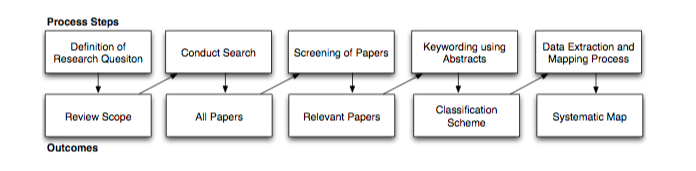
\includegraphics[width=100mm]{pic1.png}
\caption{Systematic Mapping Steps~\cite{Petersen:2008:SMS:2227115.2227123}.\label{fig:sms}}
\end{figure}

On the first step, "Definition of Research question", the questions that must be answered on the survey are defined. On "Review Scope", researchers target the papers/journal sources that will be taken into consideration on the systematic map. After that, the "Search" step is done and "All papers" are retrieved. After a initial "Screening of the papers", the "Relevant papers" are chosen according to inclusion and exclusion criteria defined by the research team. 

Instead of reading the full paper, researchers focus on reading the abstracts and keywords ("Keywording using Abstracts") to classify the papers. After that, a "Classification Scheme" is built. After matching each paper with the classification schema ("Data Extraction and Mapping Process"), the  "Systematic map" is finished. 


In the next section we build a systematic mapping database transition scenarios from relational database management systems to NoSQL scenario.


\section{A Systematic Mapping}
\label{sec:asm}

In this section we describe how our systematic map was conceived. 
Some steps of the original process were joined together on this section to simplify the outcomes comprehension.

We started by defining our research scope and by pointing out the questions that we wanted to answer in the end of the survey. After the definition of the research scope we selected the keywords that composed the boolean search string.

After we had the search string well defined we queried the chosen bibliographical databases and started the screening the papers step.

After that, we defined a classification schema and classified the relevant papers. These steps (screening of papers to classification scheme) weren't linear as shown on Figure ~\ref{fig:sms}. We had to iterate on the screened papers a few times to find the ideal classification schema to our systematic map. 

\subsection{Definition of the research questions}

As we wanted to investigate how SLAs can be used in database transitioning processes, we proposed three main research questions and two associated questions.

\paragraph*{\textbf{RQ1)} What are the reasons to change from RDBMSs to NoSQL solutions?}
\paragraph*{\textbf{AQ1.2)} What are the pros and cons to migrate from RDBMSs to NoSQL solutions?}
\paragraph*{\textbf{AQ1.2)} How can we measure the overall improvements promised by this change?}

\paragraph*{\textbf{RQ2)} How can SLAs be used to guide database transitioning processes from RDBMSs to NoSQL databases in cloud-based apps? }
\paragraph*{\textbf{RQ3)} Is there a standard representation of SLAs in cloud services?}

These are relevant questions for our survey as our focus is to determine how SLAs can be used in Database migrations scenarios. Our questions cover \textit{WHY} it is good to migrate from RDBMSs with a NoSQL solution and \textit{HOW} we can do it. 


\subsection{Definition of keywords}

Our research scope can be splitted in three main categories: 

1) Databases: As we wanted to investigate RDBMS to NoSQL transitions, we defined that a representative query string for this category would be 

\begin{center}
\textit{NoSQL AND (rdbms OR relational)}
\end{center}

2) Migration: A number of terms terms were oftenly linked with database migration and transition scenarios. Most of them, however, are consistently represented by the radicals ``migr" and ``transit". Thus the representative search string for this category is defined by: 


\begin{center}
\textit{migr* OR transit*}
\end{center}


3) Service level agreements: Service Level Agreements can also be represented by its acronym (SLA). A good search string for this category is defined as 
\begin{center}
\textit{``Service Level Agreement" OR SLA}
\end{center}

As we defined the three main categories of interest, what we wanted to survey is their conjunction. This way, the final search string can be represented as: 

\begin{center}
(migr* OR transit*) AND (NoSQL AND (rdbms OR relational)) AND (SLA OR ``Service Level agreement") 
\end{center}

\subsection{Conduct Search for Primary Studies (All Papers)}\label{sec:allPapers}

The next step of our systematic map was to identify relevant publishers. We surveyed academia experts and chose 5 main publishers: \textbf{Springer, ACM, Sciencedirect, IEEE and Elsevier}. All of these publishers have relevant publications about databases and Service Level Agreements, as they index publications from reputable international conferences.  

Each of these publishers had their own search engine, and some bugs were found on these engines while building our boolean term. IEEE, for example, returned 0 results to the query string "changes AND database AND nosql AND sla". When we searched the same query on Google Scholar filtering \textit{only IEEE publications} we found \textbf{90} results.   

To mitigate the risks of having different results for the same query on different search engines, we used Google Scholar as a meta-search engine. 

During this step, we also concluded that 2009 would be the starting year of our survey, since this was the year when the term NoSQL was reintroduced on the market, by Johan Oskarsson (Last.fm)\cite{ericevans}.

\subsection{Search Strategy}\label{sec:searchStrategy}

Google Scholar returned 74 results for our search string. We have also manually included other particularly relevant publications that were picked from selected sources, such as \cite{mastersthesrilinda}. These publications were either not published by the selected publishers or were not indexed by Google Scholar. 

It is important to mention that our scope is not limited to the list of publishers identified in \ref{sec:allPapers}; these publishers represent the minimal coverage of the literature that we can assure that are covered in this systematic map.

Our search strategy was composed by the following steps:

Step 1 - Basic Search: Search publications from 2009 to 2015 that matched the query string. This search was performed on 11 April 2015. 

Step 2 - Dump the retrieved results on a spreadsheet. This spreadsheet is publicly available on \cite{systematicMappingSpreadsheet}.

Step 3 - Reading of title and abstract: On the spreadsheet each publication has title, abstract, year and referenced URL. Title and abstract were considered on the initial screening. On this step we discarded publications that are notably not related to the topic of our study (e.g., we removed the paper intitled \textit{``Incremental dataflow execution, resource efficiency and probabilistic guarantees with Fuzzy Boolean nets"} from our survey.) 

Step 4 - Apply inclusion/exclusion criteria: The inclusion/exclusion criteria are shown below. We first applied the inclusion criteria over the selected works, and then exclusion criteria removed the out of scope publications. Only papers clearly not relevant for the purposes of the study were removed.

\begin{enumerate}
    \item Inclusion Criteria: 
    \begin{itemize}
      \item The publication is about a migration from RDBMS to a NoSQL technology;
      \item The main focus of the publication is on RDBMs or NoSQL systems;
      \item The publication makes use of a SLA.
    \end{itemize}
    \item Exclusion Criteria
	\begin{itemize}
    \item Non-english written publications;
		\item Access-restriction to the original publication;
		\item Non-technical publications;
    \item The work is about migrations within the same database DBMS;
    \item The work is not related to databases or SLAs.
    \item The work is related to databases but no comparison is made between two technologies.
    \end{itemize}
    
\end{enumerate}


Step 5 - Fast Reading of the papers: We've performed a fast read of all publications that were not excluded on the previous step. This helped us to classify each paper accurately. This step is extensively detailed on the next section. 


%$\newpage
\subsection{Classification of the Papers}

We classified each selected publication in three facets: \textbf{Contribution Type}, \textbf{Technologies used} and \textbf{SLA representation}. 


\begin{enumerate}
    \item \textbf{Contribution type}: On the initial screening of papers we have defined 5 main types of contribution to our study. Other systematic mapping studies, such as \cite{6405289} and \cite{Ameller201542} use a similar classification schema for contribution type.
    \begin{itemize}
      \item \textbf{Benchmark}
      \item \textbf{Migration Experience Report}
      \item \textbf{Bibliographical Review}
      \item \textbf{Tool}
      \item \textbf{Framework / Process}
    \end{itemize}

    When a migration of databases is described in a publication, we also classify specific data to answer the questions of this study:  Source and Target technology of the migration, motivation to migrate and ``Uses SLA or other artifact to validate the migration?"; 

    \item \textbf{Technologies used}: To classify and rank the technologies mentioned on each paper we have developed a \textit{``Batch-PDF-Tokens-Matcher"}. This tool matches a list of strings against a list of PDF files. The tool was made open-source and is publicly available on \cite{pythonBatchPDFTokenMatcher}.

    In our case, we wanted to find the most cited technologies on relevant publications. As it was not possible to include all database types on this category, we chose to match only the 250 most-popular databases, ranked by \cite{dbranking}.

    \item \textbf{SLA representation}: One of the questions that our study wanted to answer was RQ3 (Is there a standard representation of SLAs in cloud services?). There are several ways to represent an SLA, and we clusterized some of these ways. It is also possible that no information is given about SLA representation on the publication, so we added two subcategories to this facet: "No SLA is used" and "Missing information".  
    \begin{itemize}
      \item \textbf{Tool/Code/Database records}
      \item \textbf{Language}
      \item \textbf{Missing Information}
      \item \textbf{No SLA is used}
    \end{itemize}  
\end{enumerate}

A graphical representation of our classification schema is detailed on Figure~\ref{fig:classificationSchema}. We have listed only a subset of the several technology types that were found on the review.

\begin{figure}[!h]
\centering
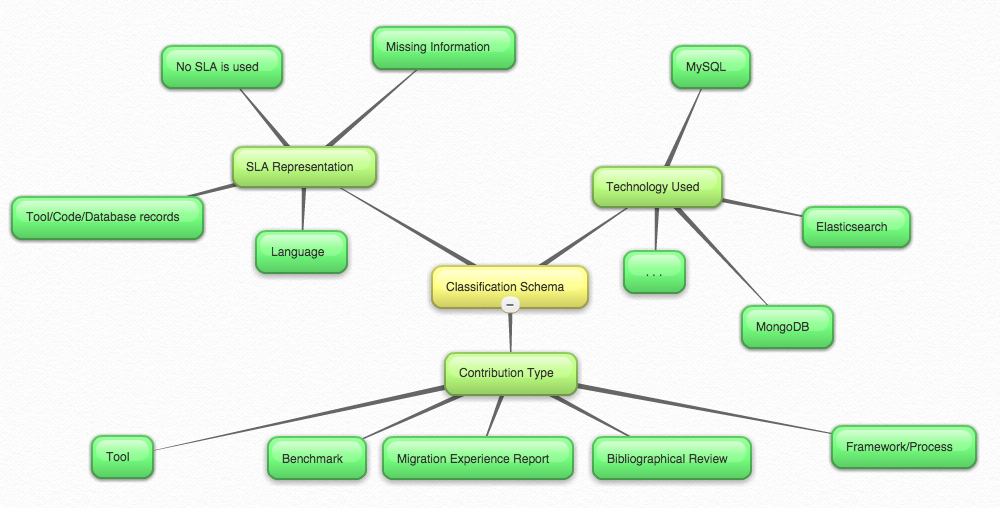
\includegraphics[width=130mm]{classificationSchema.png}
\caption{Classification scheme for selected publications \label{fig:classificationSchema}}
\end{figure}



%\newpage
\section{Outcomes}
\label{sec:outcomes}

As mentioned in Section~\ref{sec:searchStrategy}, 74 publications were found matching our query string on IEEE, Elsevier, ACM, Springer and Sciencedirect using Google Scholar as a meta-search engine. We have manually added other 3 publications to our study. These publications were either not published by the selected publishers or were not indexed by Google Scholar. 

34 out of the total of 77 publications were considered in our study. A column was added in the spreadsheet to justify the rejection of each rejected publication.

The considered publications are: \cite{6665220} \cite{6253526}  \cite{6461875} \cite{6597164} \cite{6616442} \cite{Xiong:2012:DMR:2213598.2213614} \cite{Alomari:2014:CFD:2684200.2684324} \cite{6632740} \cite{6253597} \cite{cloudhosteddatabases} \cite{6655733} \cite{192837618237651293} \cite{6616442} \cite{designinganddevelopment} \cite{5959767} \cite{Petcu20131417} \cite{Giannikis:2013:WOU:2463676.2463678} \cite{1236781237} \cite{6280329} \cite{6681233} \cite{Xiong:2011:APA:2038916.2038931} \cite{7037676} \cite{7017947} \cite{Qiao:2013:BFE:2463676.2465298} \cite{5742778} \cite{Montes20132026} \cite{Elmore:2013:CTB:2463676.2465308} \cite{12789361729836} \cite{6842585} \cite{Shue:2014:ARV:2592798.2592823} \cite{Schram:2012:MND:2384716.2384773} \cite{buazuartransition} \cite{gomez2014building} \cite{6546068}


The results are given in two steps: \textit{Frequency Analysis between relevant criteria} and \textit{Answers to research questions}. 

\subsection{Frequency Analysis between relevant criteria}
\label{frequencyAnalysis}

Each analysis is presented below and is followed by a brief interpretation of the result. 



\begin{itemize}
\item{Publications by year: }
The publications by year table shows us that it was in 2013 when most of the publications were made on this research area. As we still haven't reached  the middle of 2015 it is expected that not many publications are indexed on the search engines on this year.
\begin{figure}[htb!]
\centering
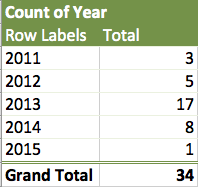
\includegraphics[width=30mm]{graph2.png}
\caption{Publications by year}
\end{figure}



\item {Frequency - Publication type vs Years: }
An interesting patter can be found on the table of Publication Type vs Years; ``Migrations Experience Reports" were one of the main focus of this paper, but only 3 publications of this type were found on our systematic map, however. 

\begin{figure}[htb!]
\centering
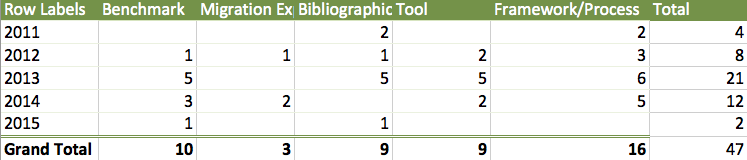
\includegraphics[width=100mm]{graph1.png}
\caption{Frequency - Publication type vs Years}
\end{figure}


\item{Publications by country: }
USA, Australia and Romania were responsible for almost 50\% of the total selected publications. The other half of publications were distributed among other 16 countries, proving that the research area is not being developed by a single research group. 
\begin{figure}[htb!]
\centering
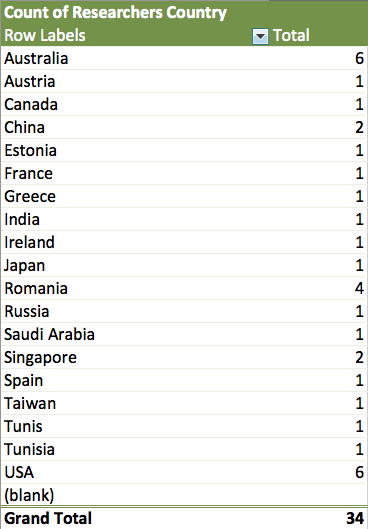
\includegraphics[width=50mm]{graph3.png}
\caption{Publications by country}
\end{figure}



\item{Popular Technologies: }
Cassandra, MongoDB and MySQL were the most-cited databases on the papers that we analyzed. This chart might be used as a starting point to propose innovative works in the area of database migration. The full JSON is available on \cite{fullDBJson}.
\begin{figure}[htb!]
\centering
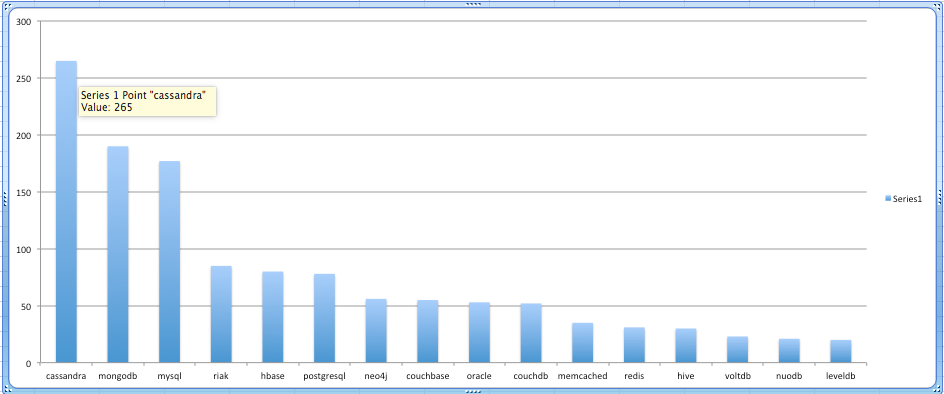
\includegraphics[width=150mm]{database_count.png}
\caption{Most-cited database technologies.}
\end{figure}

\item{SLA Representation: }
29\% of the publications didn't make any use of SLAs. Another big part - 32\% - didn't even mention how the SLA is represented internally. 3 publications propose or use DSLs (Domain Specific Languages) to represent SLAs. This evidences a clear absense of standards when defining/using SLAs. The full table is presented below.  \cite{fullDBJson}.
\begin{figure}[htb!]
\centering
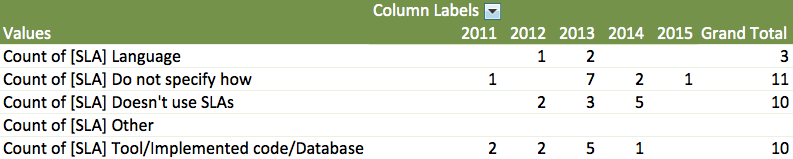
\includegraphics[width=100mm]{graph4.png}
\caption{SLAs representation.}
\end{figure}



\end{itemize}


\newpage

\subsection{Answers to research questions}

In this mapping study we have surveyed the state of the art in transitions from RDBMSs to NoSQL databases. We created a rigorous protocol which analyzed 77 publications to answer the research questions that we identified previously. We may consider the answer to these questions as the main outcome of this paper. The answers are summarized below:
\\

{\textbf{(RQ1) and (AQ1.2)} investigate the motivation of a database transition. We found a number of reasons to migrate from a relational database to a NoSQL/Hybrid model. As the migration is most of the time motivated by the benefits of these models, the answer to the questions RQ1 and AQ1.2 is presented together. 

 The main publications that reference the benefits and disadvantages of NoSQL / Hybrid solutions  were \cite{Schram:2012:MND:2384716.2384773} \cite{buazuartransition} and \cite{gomez2014building}.

\begin{enumerate}
    \item Benefits: 
\begin{itemize}
  \item Segments of the data to be read and processed in parallel using a MapReduce framework, such as Hadoop;
  \item Schema-less data model;
  \item Support for large files;
  \item Scalability - relational databases tend to ``Scale up", which is opposed to the ``Scale horizontally" strategy used by hybrid solutions;
\end{itemize}

    \item Disadvantages:
    \begin{itemize}
    \item A big disadvantage on moving from a RDBMS to a NoSQL/Hybrid solution is the need for changes on the data models of the application. Several publications address this problem, such as \cite{Schram:2012:MND:2384716.2384773} \cite{Cattell:2011:SSN:1978915.1978919} and \cite{Mohan:2013:HRI:2452376.2452378}
    \item Another disadvantage of NoSQL and Hybrid solutions is the fact that these concepts are relatively new. As we mentioned previously, the term NoSQL was used to reference these types of databases for the first time in 2009\cite{ericevans}. The relational model has been in use for more than 30 years;As it is a new concept, it is particularly hard to find developers with a large experience in NoSQL databases.
\end{itemize}
    

\end{enumerate}


{\textbf{(AQ1.2)} How can we measure the overall improvements promised by this change?

No publication was found addressing the problem of measuring the overall improvements after a database transition. In fact, as it is shown on \ref{frequencyAnalysis}, there are few publications with the ``Migration Experience Report"  type. 

Several benchmarking frameworks, such as TPC-H, TPC-DS and YCSB were discovered\cite{6616442} during our survey, though. These benchmarking frameworks could be a good starting point to develop new tools and specialized frameworks to solve this problem. This seems to be a promissing research theme for future works.

\paragraph*{\textbf{RQ2)} How can SLAs be used to guide database transitioning processes from RDBMSs to NoSQL databases in cloud-based apps? }

A number of works were found relating SLAs with Quality of Service (QoS) and Quality of Experience (QoE). Several publications, such as \cite{Xiong:2012:DMR:2213598.2213614}, \cite{Konstantinou:2012:TEN:2213836.2213943} and \cite{Klems:2012:RQM:2477172.2477488} propose a SLA-centric approach to monitor and control the performance of cloud-based apps. 
\cite{6253526}, \cite{6461875}, \cite{6511780} and \cite{Xiong:2011:APA:2038916.2038931} propose SLA-centric/User-Centric solutions to monitor the performance of web applications. All these solutions are technology-agnostic and could be used to monitor the performance improvements promised by a database transitioning process.

The question RQ2 was subject of discussion with industry experts and it was found out that there are some services, such as New Relic~\cite{newrelic}, Appsee~\cite{appsee} and Datadog~\cite{datadog} that provide SLA-monitoring tools for web apps.


\paragraph*{\textbf{RQ3)} Is there a standard representation of SLAs in cloud services? }

The selected publications did not present a standardized and common representation for SLAs. In fact, 32\% of the selected publications did not even mention how the SLA was represented. 29\% represented the SLAs as tables/documents stored on databases without any sla-oriented guidelines. This evidences a clear absense of standards when defining/using SLAs.

\cite{6546068} proposes SYBL: \textit{An Extensible Language for Controlling Elasticity in Cloud Applications. SYBL allows specifying in detail elasticity monitoring, constraints, and strategies at different levels of cloud applications, including the whole application, application component, and within application component code. Based on simple SYBL elasticity directives, our runtime system will perform complex elasticity controls for the client, by leveraging underlying cloud monitoring and resource management APIs.}

Some other initiatives that tried to define the mechanisms by which Webservice SLAs are stablished are WS-Agreement \cite{citeulike:2805191} and WSLA \cite{4578560}. Also, \cite{5547150} presents a framework for managing the mappings of the Low-level resource Metrics to High-level SLAs (LoM2HiS framework). 
9

It is obvious that future works on standardizing the representations of SLAs are needed. 

\section{Conclusions}
By analyzing the charts and the answers to the research questions we can conclude that the research area of this mapping study is still not mature. 

There is a lack of consensus and standards on this research area, as no official guidelines for migrating from a relational database to a NoSQL/Hybrid database were found. It was also not found a standard way to represent and create SLAs. These two points seems to be promising research topics and will be covered on future works.


%\newpage
\bibliographystyle{plain}
\bibliography{systematicMapping}	

\end{document}